% ANL Beamer template
\documentclass[aspectratio=169]{beamer}
\usepackage[english]{babel}
\usepackage[utf8]{inputenc}

% AMSLaTeX packages
\usepackage{amsthm}
\usepackage{amsmath}
\usepackage{amsfonts}
\usepackage[algoruled]{algorithm2e}

\usetheme{default}
\useoutertheme{default}
% we want to use images
\usepackage{graphicx}
\usepackage{movie15}
\usepackage{hyperref}

% table relates packages
\usepackage{booktabs}
\usepackage{multirow}
% pick a font
\usepackage{palatino}           
% \usepackage{times}
\usepackage{tikz}
\usetikzlibrary[positioning,arrows,decorations.pathmorphing,backgrounds,fit,calc]
% \AtBeginSection[]  % "Beamer, do the following at the start of every section"
% {
%   \begin{frame}<beamer> 
%     \frametitle{Outline} % make a frame titled "Outline"
%     \tableofcontents[currentsection]  % show TOC and highlight current section
%   \end{frame}                    
% }

% \AtBeginSubsection[]
% {
%   \begin{frame}
%     \frametitle{Outline}
%     \tableofcontents[currentsection,currentsubsection]
%   \end{frame}
% }

\AtBeginSection[]
{
   \begin{frame}
       \frametitle{Outline}
       \tableofcontents[currentsection]
   \end{frame}
}

\newcommand{\ebox}[1][1em]{\framebox[#1]{\phantom{M}}}

\setlength\arraycolsep{1.4pt}% some length

%gets rid of navigation symbols
\setbeamertemplate{navigation symbols}{}

%gets rid of bottom navigation bars
\setbeamertemplate{footline}[page number]{}
\setbeamertemplate{headline}{}


\usebackgroundtemplate{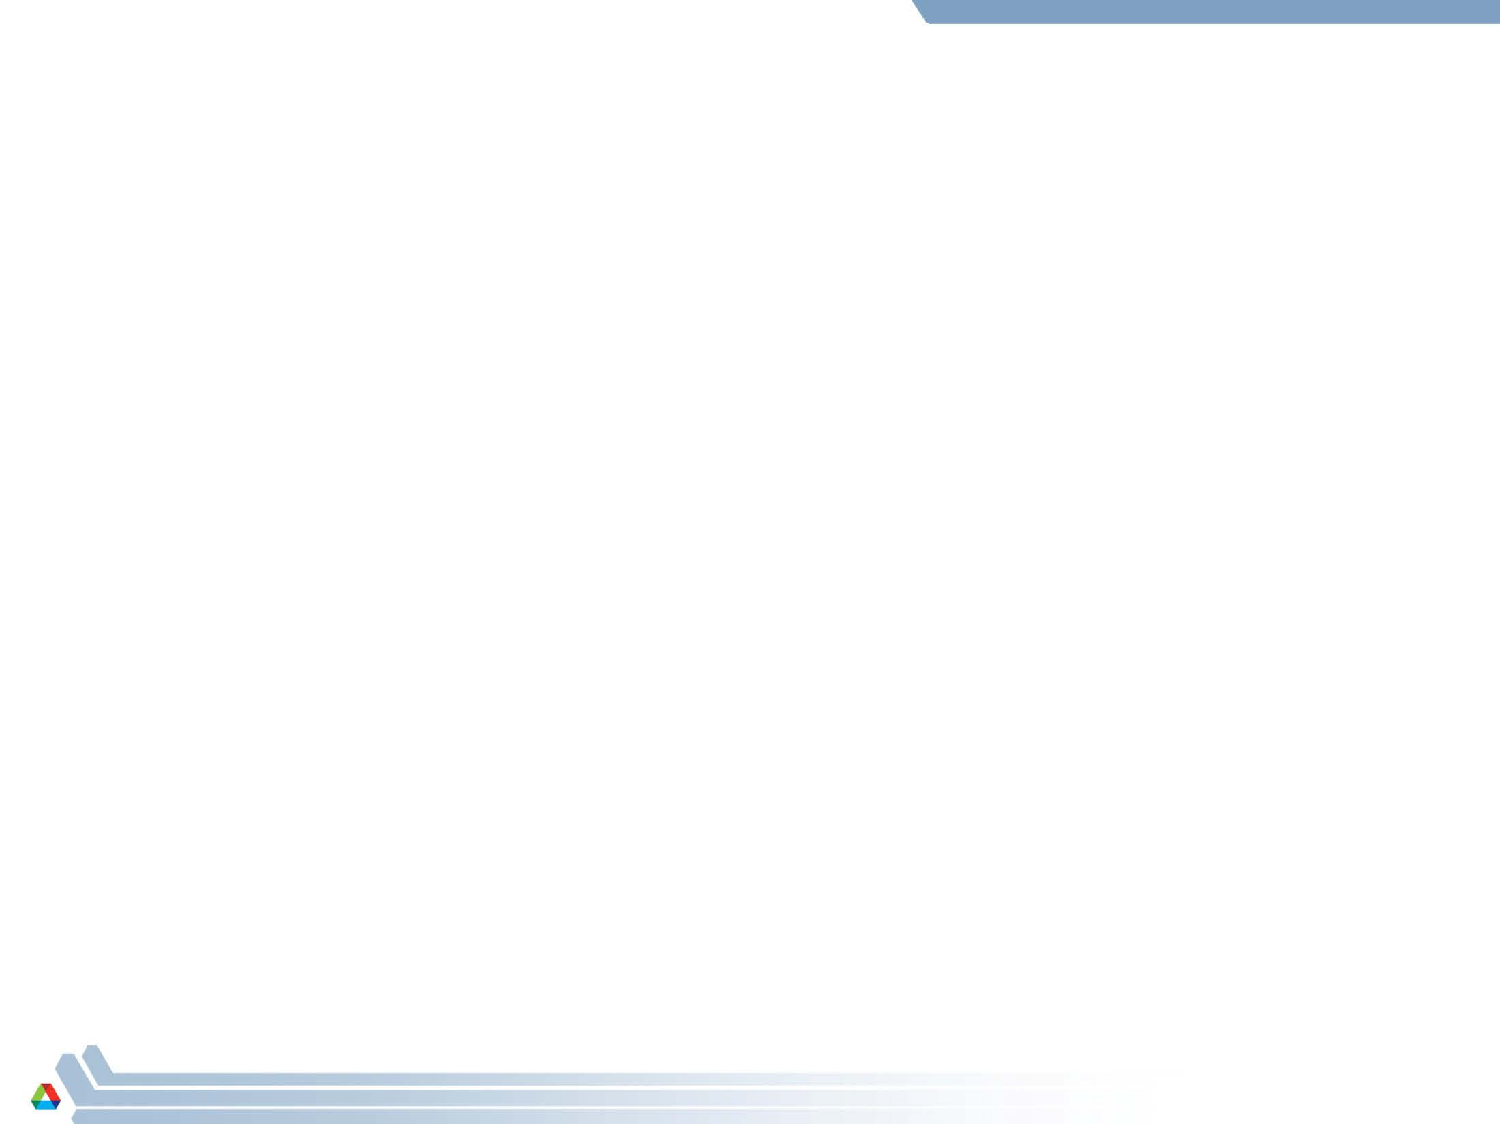
\includegraphics[width=\paperwidth]{../templates/NormalANLBlue}}

% Define big arrow down
\newcommand{\xdownarrow}[1]{%
  {\left\downarrow\vbox to #1{}\right.\kern-\nulldelimiterspace}
}

\usepackage{xcolor,ulem}

\AtBeginSection[]{
  \begin{frame}
  \vfill
  \centering
  \begin{beamercolorbox}[sep=8pt,center,shadow=true,rounded=true]{title}
    \usebeamerfont{title}\insertsectionhead\par%
  \end{beamercolorbox}
  \vfill
  \end{frame}
}

% Title/author info
\title{Geometric Considerations when Surrogate Modeling for Multiobjective Optimization}
\subtitle{\onslide<2>{The Geometry of a Bad Dataset}}
\author{Tyler Chang$^a$, Manisha Garg$^{a,b}$, and Stefan Wild$^a$}
\institute{$^a$MCS Division, Argonne National Laboratory

$^b$Dept.\ of Mathematics, Univ.\ Illinois Urbana Champaign}
\date{\small SIAM MDS 2022}

% Slides start here
\begin{document}

% Set the background graphics
\setbeamertemplate{footline}{}
{
\usebackgroundtemplate{
\includegraphics[width=\paperwidth]{../templates/TitleANLBlue}}
\frame{\titlepage}
}
\setbeamertemplate{footline}[page number]{}

% FRAME: overview
\begin{frame}
  \frametitle{Outlines}
  \tableofcontents
\end{frame}

% ========================================
% main slides come here
% ========================================

\section{Problem Setting and Some Background}

\begin{frame}\frametitle{Multivariate Interpolation}
\begin{columns}
\begin{column}{.35\textwidth}
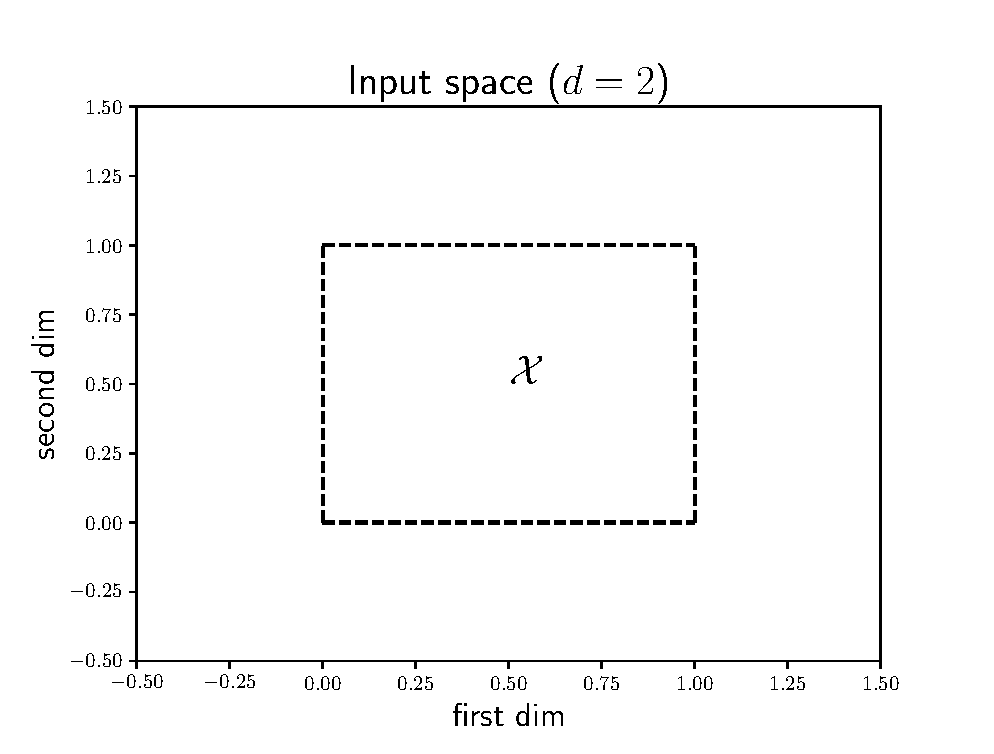
\includegraphics[width=\textwidth]{feasible_design.eps}
\end{column}
\begin{column}{.2\textwidth}
\begin{center}
$\xrightarrow{\hspace*{2cm}}$
$$
F : {\cal X} \rightarrow {\cal Y}
$$
\end{center}
\end{column}
\begin{column}{.35\textwidth}
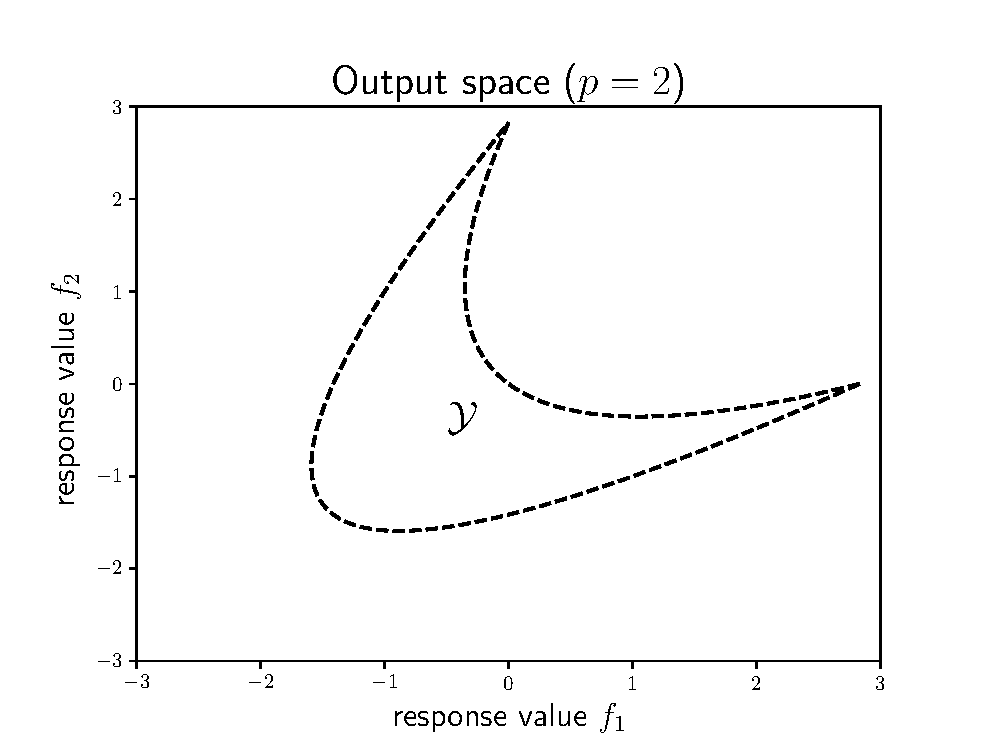
\includegraphics[width=\textwidth]{convex_pareto.eps}
\end{column}
\end{columns}
\bigskip
\bigskip
\bigskip
\end{frame}

\begin{frame}\frametitle{Multivariate Interpolation}
\begin{columns}
\begin{column}{.35\textwidth}
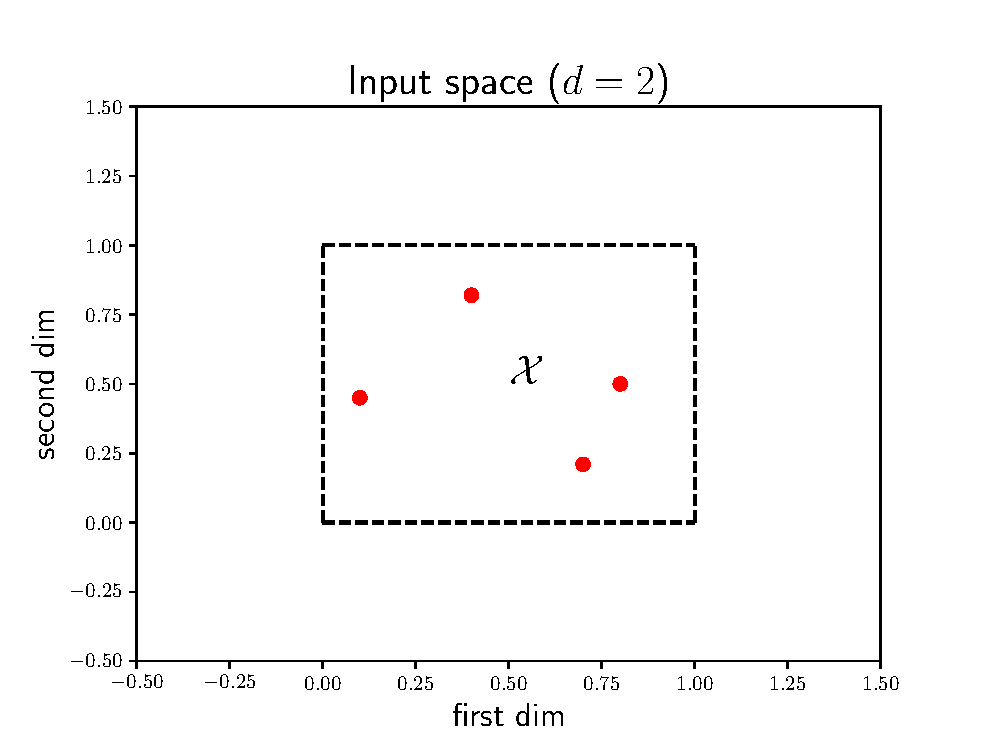
\includegraphics[width=\textwidth]{feasible_design_with_data.eps}
\end{column}
\begin{column}{.2\textwidth}
\begin{center}
$\xrightarrow{\hspace*{2cm}}$
$$
F : {\cal X} \rightarrow {\cal Y}
$$
\end{center}
\end{column}
\begin{column}{.35\textwidth}
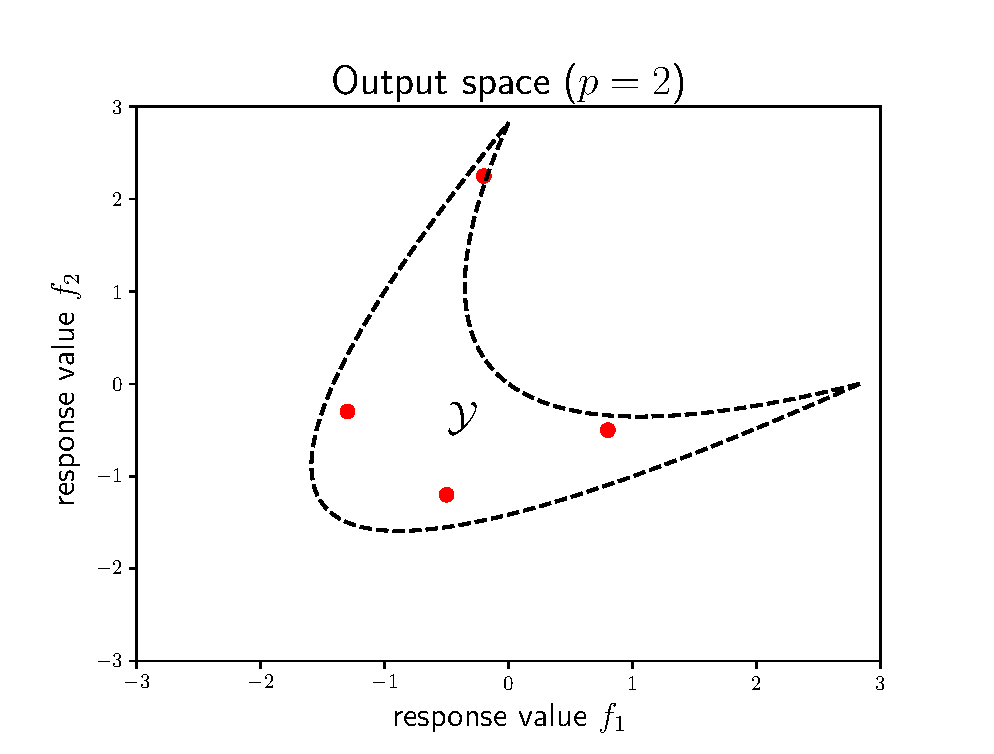
\includegraphics[width=\textwidth]{convex_pareto_with_data.eps}
\end{column}
\end{columns}

\pause
\bigskip

{\large Given a set of $n$ points {\color{red} ${\cal P}$} in ${\cal X}$,
find
${\color{blue} {\hat F}} \approx F$ such that ${\hat F}({\color{red} x}) = F({\color{red} x})$ for all
{\color{red}$x\in{\cal P}$}}

\pause
\bigskip

{\large Suppose ${\cal X} \subset \mathbb{R}^d$ and
${\cal Y} \subset \mathbb{R}^p$, and $F$ is continuous
}

\end{frame}

\begin{frame}\frametitle{My Motivation: Multiobjective RSM}
\begin{columns}
\begin{column}{0.4\textwidth}
\begin{center}
\onslide<2->{
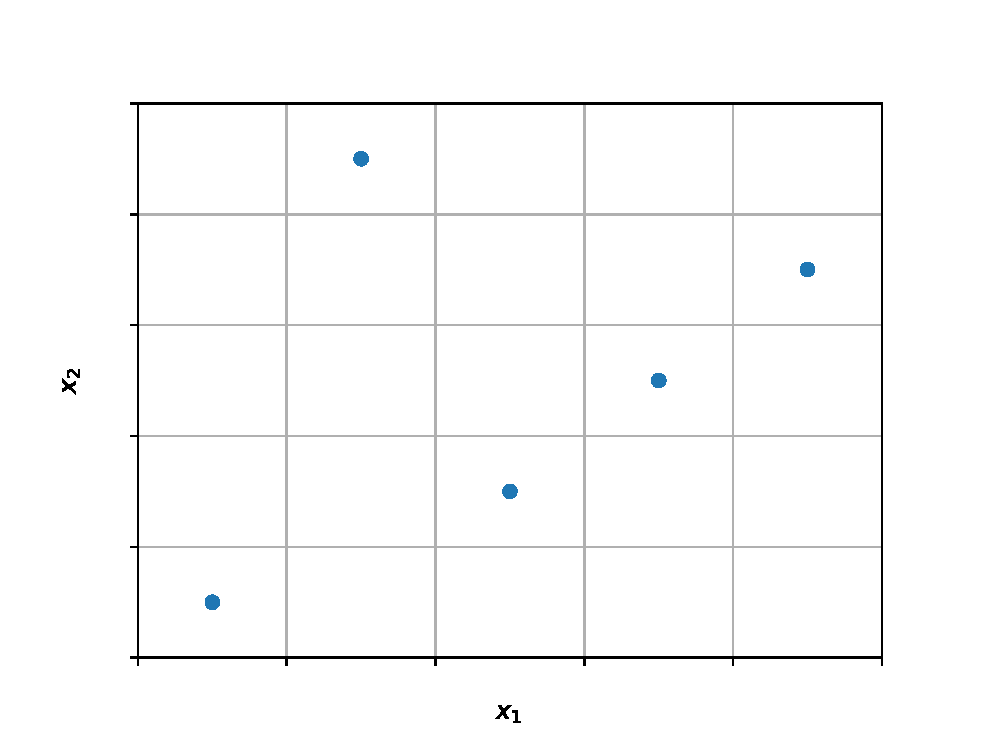
\includegraphics[width=0.6\textwidth]{lh_doe.eps}\\
}
\medskip
\vskip 0.5cm
\medskip
\onslide<5->{
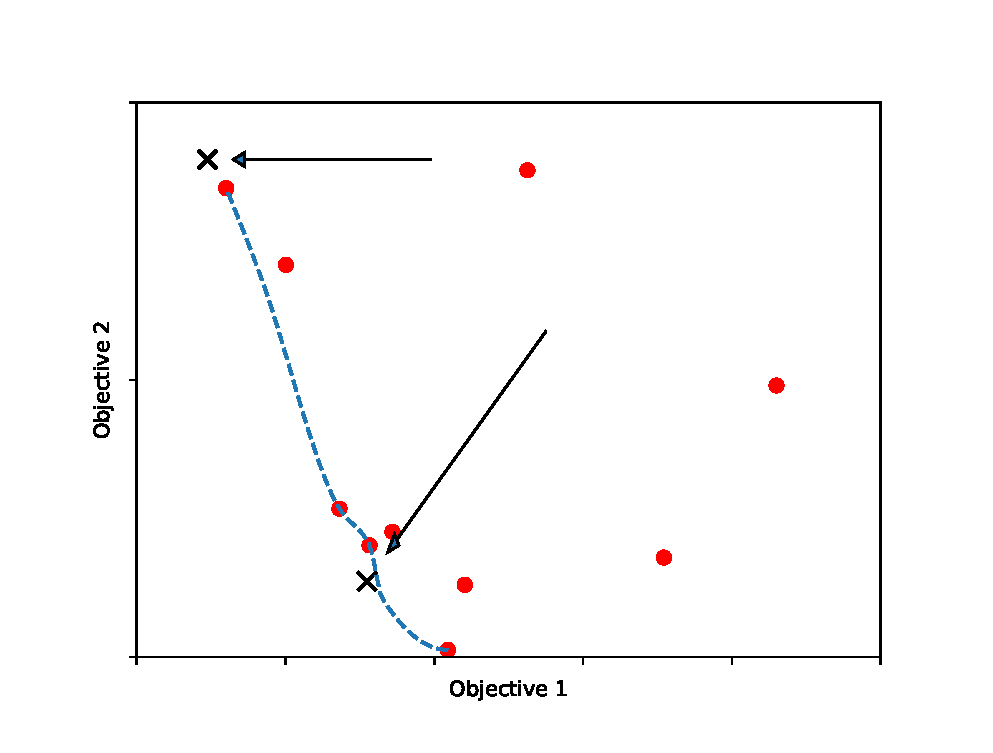
\includegraphics[width=0.6\textwidth]{tradeoff.eps}
}
\end{center}
\end{column}
\begin{column}{0.2\textwidth}
\begin{center}
\onslide<3->{
$\xrightarrow{\hspace*{1.5cm}}$}\\
\vskip 1.2cm
\onslide<6->{
$\qquad\qquad\nearrow$\\
{\Huge $\mathcal{C}$}\\
$\nearrow\qquad\qquad$}\\
\vskip 1cm
\onslide<5->{
$\xleftarrow{\hspace*{1.5cm}}$}
\end{center}
\end{column}
\begin{column}{0.4\textwidth}
\begin{center}
\onslide<3->{
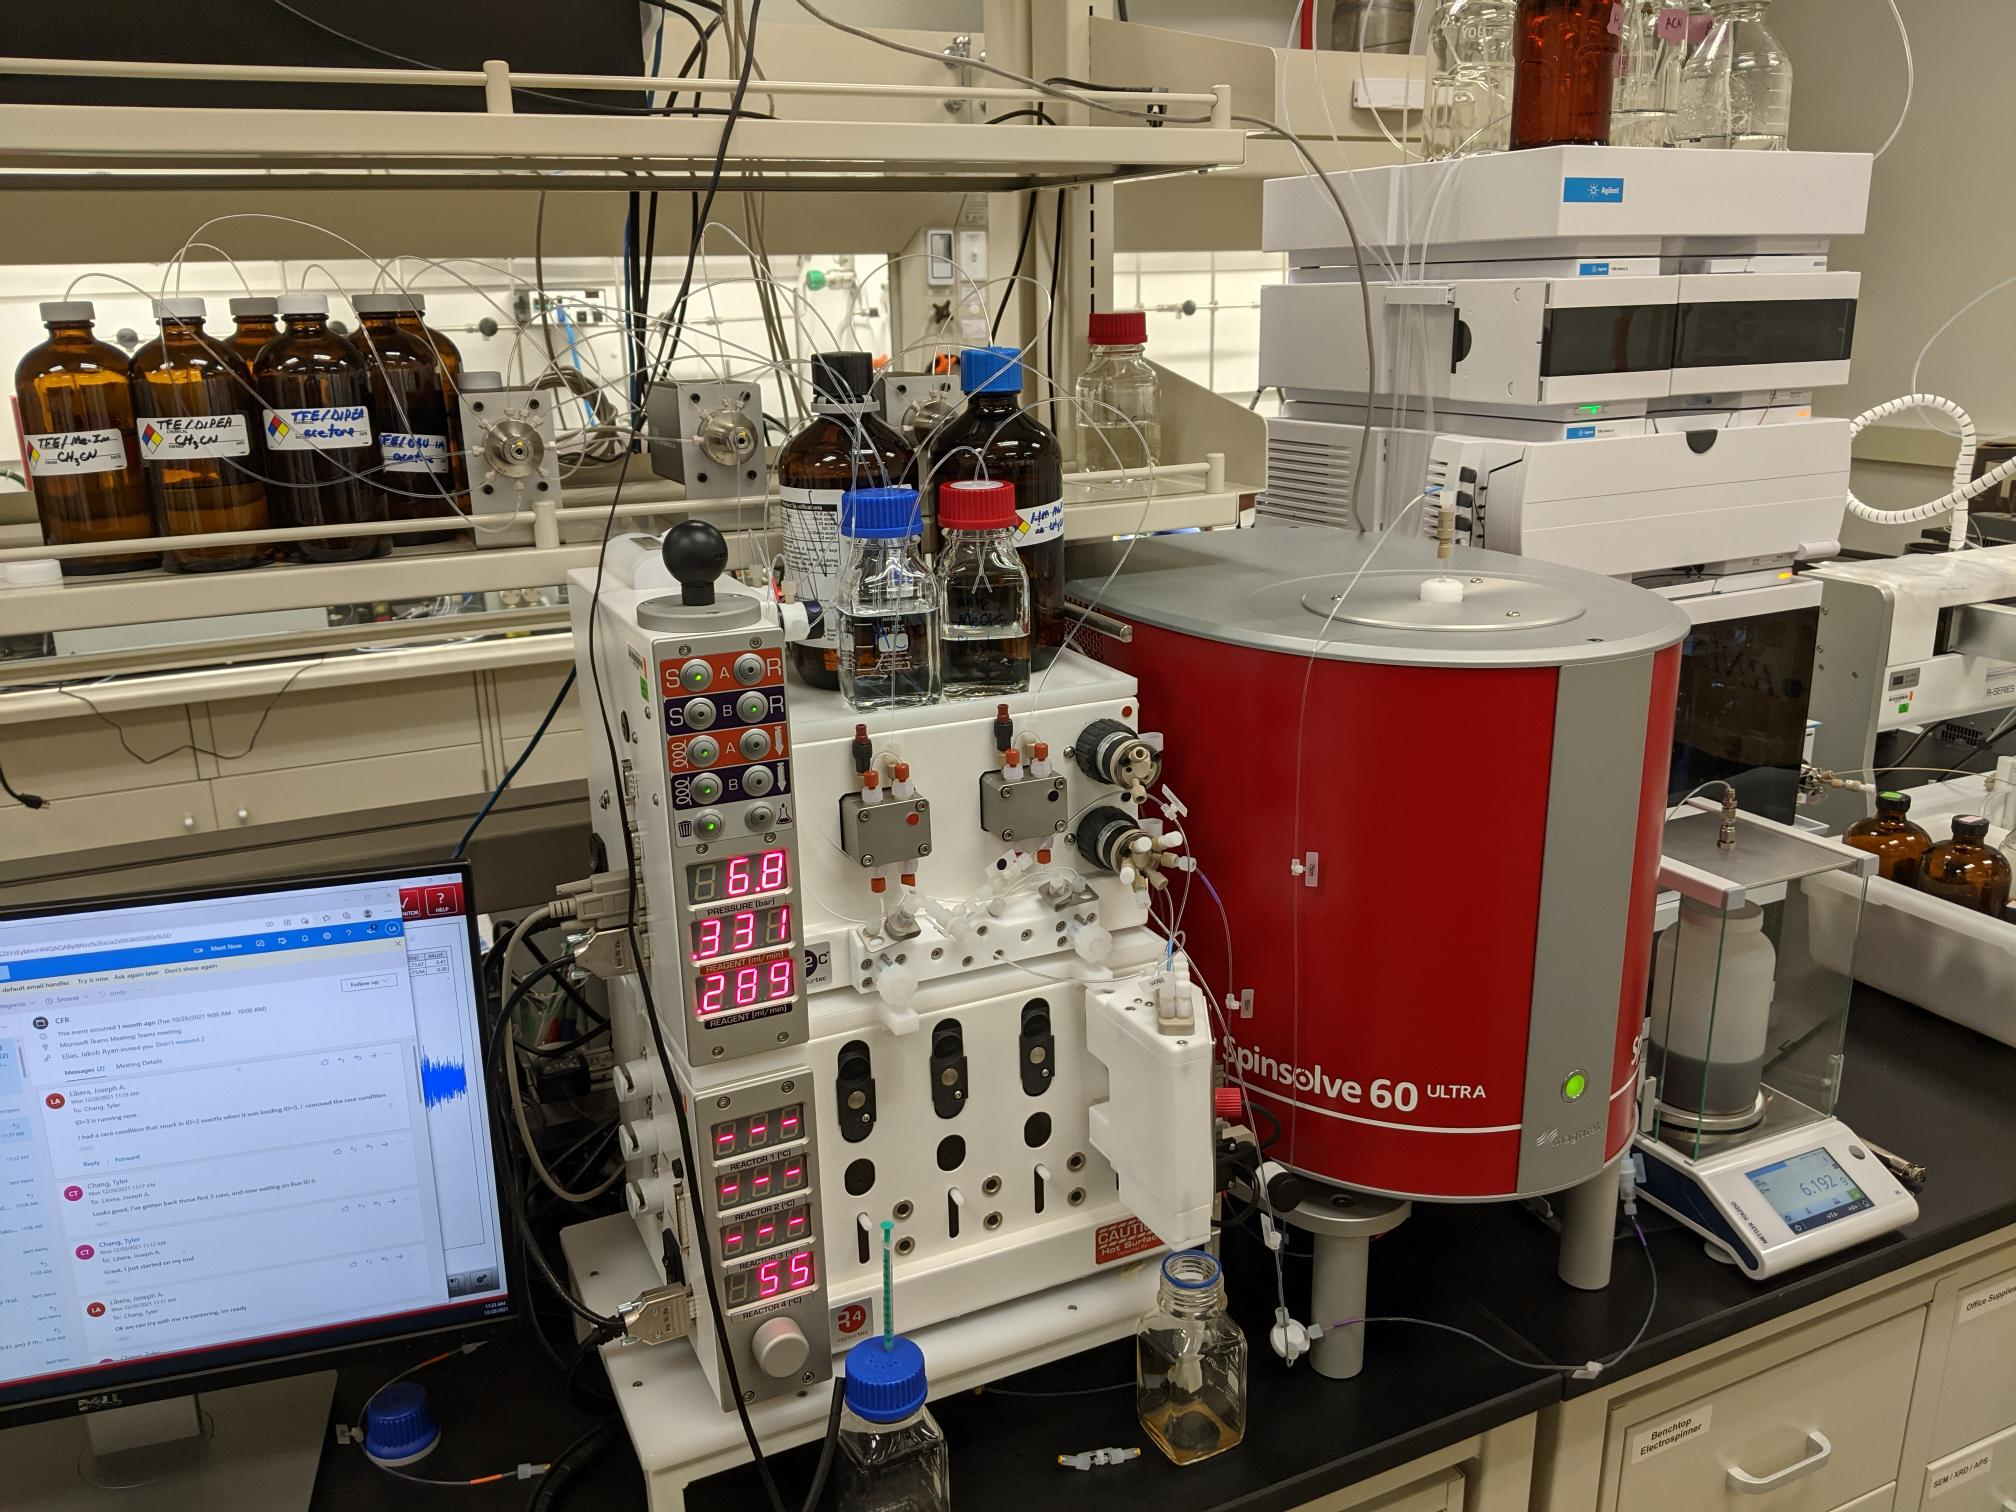
\includegraphics[width=0.58\textwidth]{lab_setup.jpg}\\
}
\medskip
\onslide<4->{
$\xdownarrow{0.5cm}$\\
\medskip
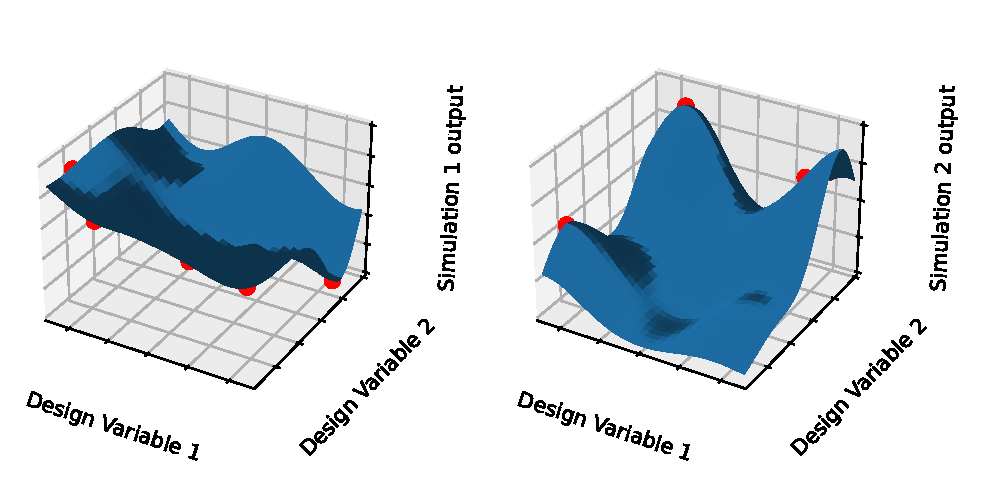
\includegraphics[width=0.9\textwidth]{rsm.eps}
}
\end{center}
\end{column}
\end{columns}
\onslide<7>{\tt https://github.com/parmoo/parmoo}
\end{frame}

\begin{frame}{Interpolation Techniques}

\begin{itemize}
\pause \item Train a neural network to 0 training error
\begin{itemize}
\pause \item For example, a fully-connected ReLU net
\end{itemize}
\bigskip
\pause \item Other statistics/machine learning models
\begin{itemize}
\pause
\item Gaussian processes
\item Support vector regressor
\item Decision tree-based methods
\end{itemize}
\bigskip
\pause \item ``Classical'' interpolation techniques
\begin{itemize}
\pause \item Polynomial interpolation
\item B-spline interpolation
\item RBF interpolants
\item generalized Shepard's methods
\item {\bf Piecewise linear interpolation}
\end{itemize}
\end{itemize}
\end{frame}

\section{My Story with Interpolation Methods}

\begin{frame}{Piecewise Linear Interpolation}
\begin{columns}
\begin{column}{0.7\textwidth}
\begin{itemize}
\item Let ${\color{blue} \cal T}({\cal P})$ be a
$d$-dimensional triangulation of ${\cal P}$.
\item Given an interpolation point $q \in {\cal CH}({\color{red} \cal P})$,
let ${\color{blue} \cal S}$ be a simplex in ${\color{blue} \cal T(P)}$
with vertices {\color{blue} $s_1$, $\ldots$, $s_{d+1}$} such that
$q\in {\color{blue} \cal S}$.
\item Then there exist unique {\it convex weights}
{\color{red} $w_1$, $\ldots$, $w_{d+1}$} 
such that $q = \sum_{i=1}^{d+1} {\color{red} w_i} {\color{blue} s_i}$.
\end{itemize}
\pause
\bigskip
Define:
$$
\hat{F}_{\color{blue} \cal T} (q) =
F({\color{blue} s_1}) {\color{red} w_1} +
F({\color{blue} s_2}) {\color{red} w_2} +
\text{ $\ldots$ } +
F({\color{blue} s_{d+1}}){\color{red} w_{d+1}}
$$
\end{column}
\begin{column}{0.3\textwidth}
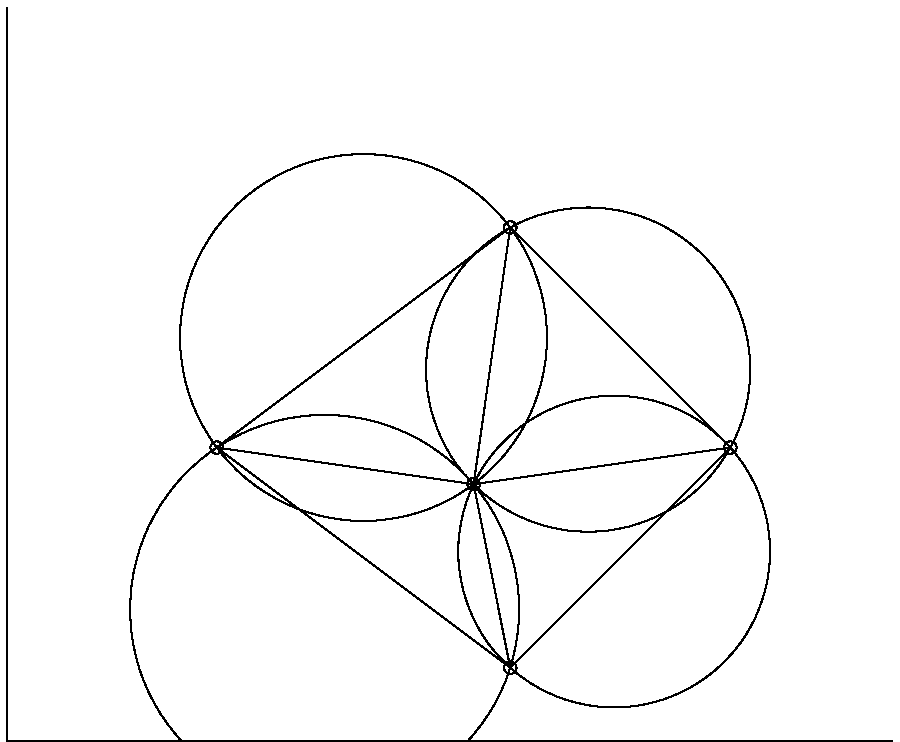
\includegraphics[width=\columnwidth]{delaunayplane-eps-converted-to.pdf}
\end{column}
\end{columns}

\pause

\vfill

{\small \it {\bf Chang} et al. 2020. Algorithm 1012: DELAUNAYSPARSE. ACM TOMS 46(4), Article No.~38.}

\end{frame}

\begin{frame}\frametitle{Error Rates for Piecewise Linear Interpolants}
For an individual component function $F_i$:
\begin{itemize}
\item Let $\nabla F_i$ be $\lambda$-Lipschitz in the $2$-norm\\
\item For ${\cal S}\in {\cal T}$ containing $q$,
\begin{itemize}
\item let $\xi$ be the diameter of ${\cal S}$ and
\item $\kappa_{\cal S}$ be the condition number of ${\cal S}$'s
barycentric transformation matrix
\end{itemize}
\end{itemize}
\pause
\bigskip
Then
$$
|F_i(q) - {\hat F}_{\cal T}(q)| \leq
{\color{blue} \frac{\lambda}{2}(1 + \sqrt{d}{\color{red}\kappa_{\cal S}})}
{\color{red} \xi^2}
$$

\bigskip

\pause

\vfill

{\small \it Lux, Watson, {\bf Chang}, et al. 2021. Interpolation of sparse high-dimensional data. Numerical Algorithms 88(1), 281--313.}

\end{frame}

\begin{frame}\frametitle{Issues Solving Real-World Problems}

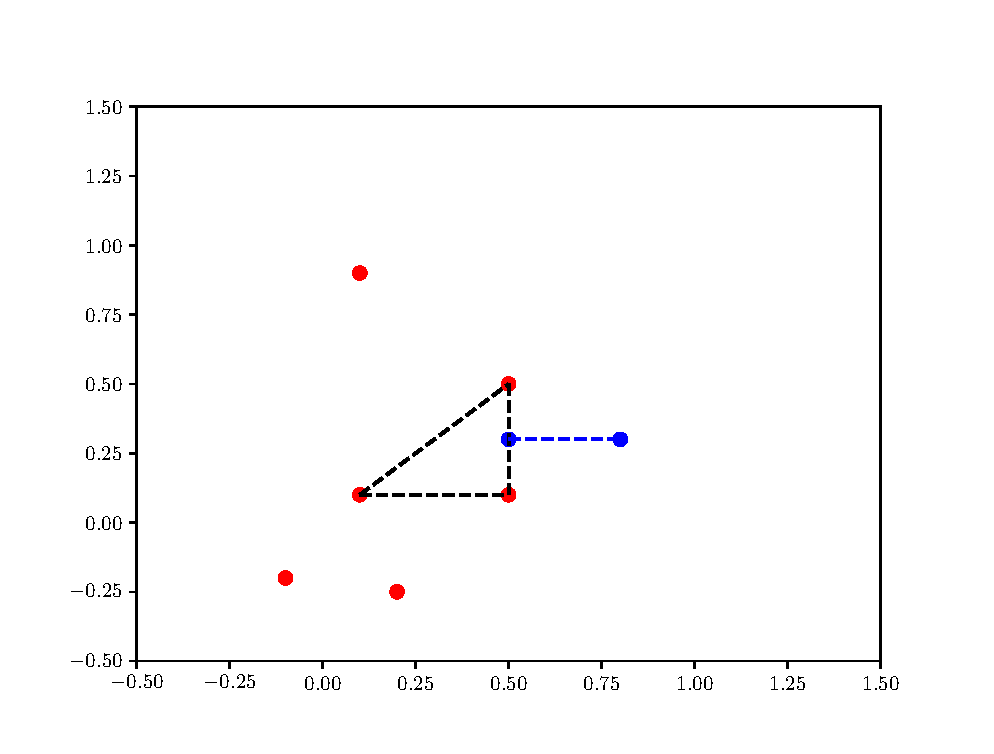
\includegraphics[width=0.3\textwidth]{ch-proj.eps}
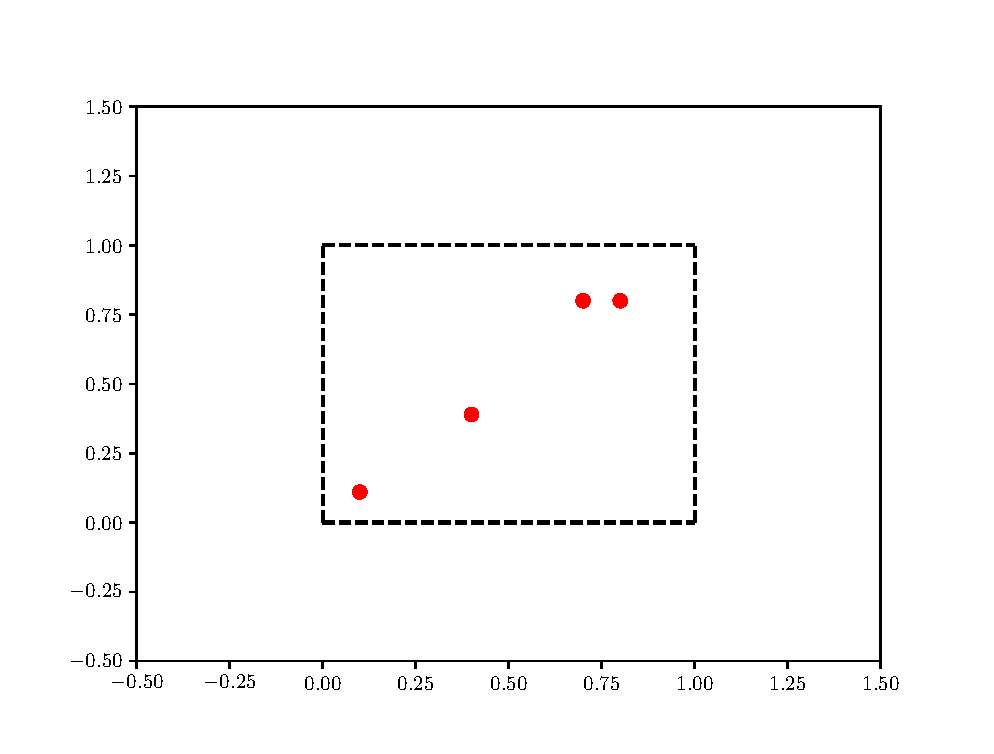
\includegraphics[width=0.3\textwidth]{poor-condition-data.eps}
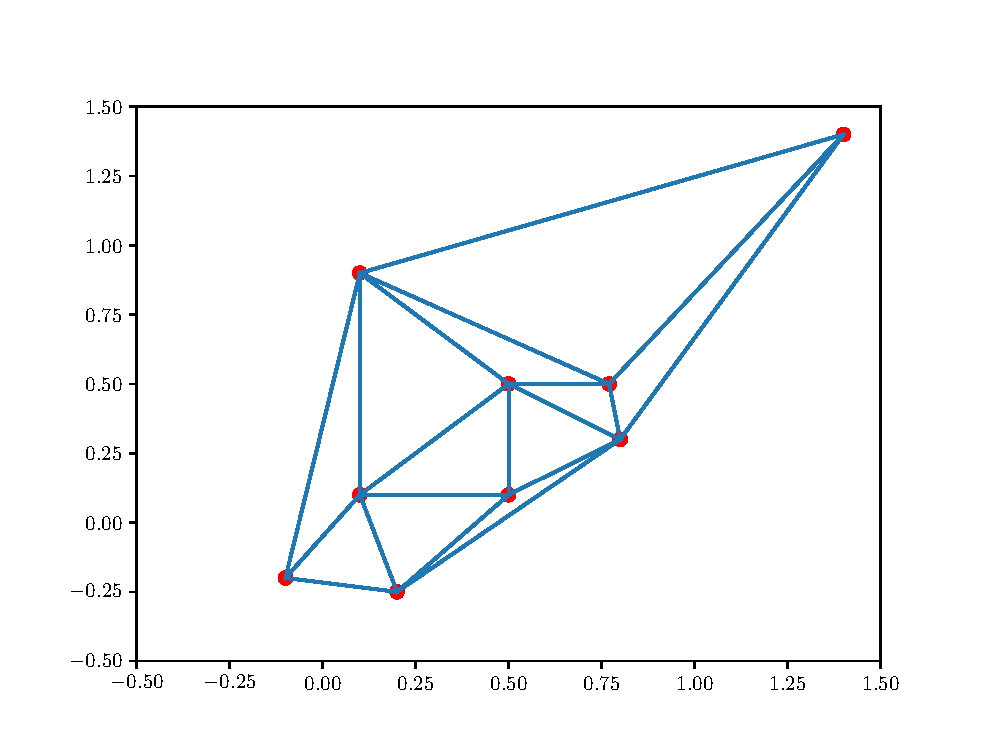
\includegraphics[width=0.3\textwidth]{unbalanced-simps.eps}

\begin{itemize}
\pause \item Too many extrapolation points (information lost in projection)
\pause \item ``Flat'' data set -- cannot (accurately) triangulate
\pause \item Several massive simplices (high error-rate, poor conditioning)
\end{itemize}

\end{frame}

\begin{frame}\frametitle{What does the theory say?}

\pause

{\small \it Gorban et al.\ 2017. Stochastic separation theorems.
Neural Networks 94, 255-259.}

\pause
\bigskip

My take:

Let ${\cal P}$ be randomly sampled by a distribution $\mu$,
then
\pause
$$
\mathbb{E}\left[ \text{vol}({\cal CH}({\cal P})) \right] \rightarrow 0
\text{ as $d$ increase}
\pause
\quad
\text{(exponentially)}
$$

\end{frame}

\begin{frame}\frametitle{But does it happen in practice?}

\pause

{\small \it Yousefzadeh 2020. Deep learning generalization and the convex hull
of training sets.
Deep Learning through Info.~Geom.~Workshop, NeurIPS.
}

\pause
\bigskip

My take:

Yes, it does... and it's bad.

\end{frame}

\section{The Geometry of Bad Data}

\begin{frame}\frametitle{Error Rates for Piecewise Linear Interpolants}
For an individual component function $F_i$:
\begin{itemize}
\item Let $\nabla F_i$ be $\lambda$-Lipschitz in the $2$-norm\\
\item For ${\cal S}\in {\cal T}$ containing $q$,
\begin{itemize}
\item let $\xi$ be the diameter of ${\cal S}$ and
\item $\kappa_{\cal S}$ be the condition number of ${\cal S}$'s
barycentric transformation matrix
\end{itemize}
\end{itemize}
\bigskip
Then
$$
|F_i(q) - {\hat F}_{\cal T}(q)| \leq
{\color{blue} \frac{\lambda}{2}(1 + \sqrt{d}{\color{red}\kappa_{\cal S}})}
{\color{red} \xi^2}
$$

\bigskip

\vfill

{\small \it Lux, Watson, {\bf Chang}, et al. 2021. Interpolation of sparse high-dimensional data. Numerical Algorithms 88(1), 281--313.}

\end{frame}

\begin{frame}\frametitle{What Could Go Wrong: Poor data conditioning}
\begin{columns}
\begin{column}{0.6\textwidth}
\begin{itemize}
\pause
\item Simplices are long and narrow
\item {\color{red} $\kappa_{\cal S}$ term blows up}
\item ${\hat F}_{\cal T}$ is hard to compute and low accuracy
\item Ex: data lies close to a lower-dimensional manifold
\end{itemize}
\end{column}
\begin{column}{0.4\textwidth}
\begin{center}
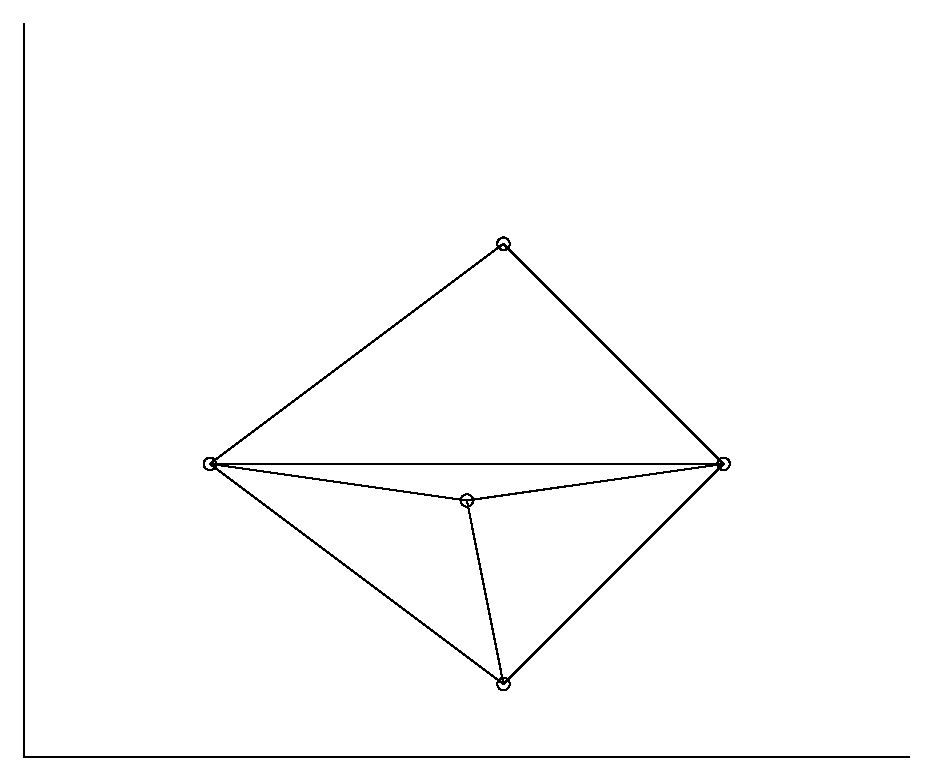
\includegraphics[width=0.6\textwidth]{triangleplane.eps}\\

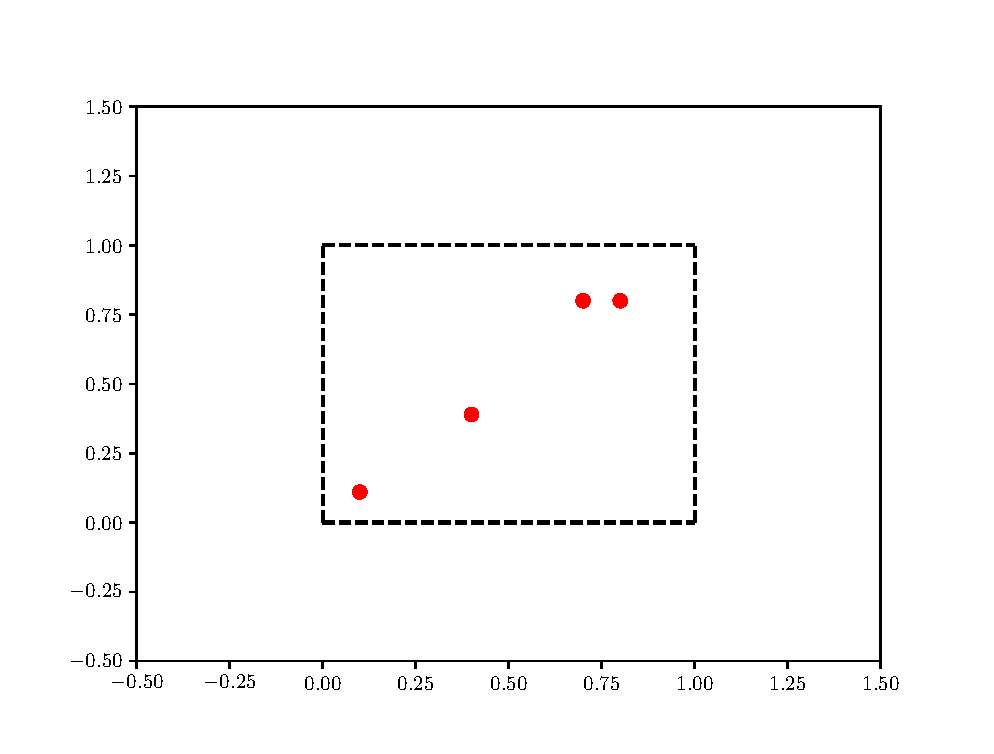
\includegraphics[width=0.9\textwidth]{poor-condition-data.eps}
\end{center}
\end{column}
\end{columns}
\end{frame}

\begin{frame}\frametitle{What Could Go Wrong: Data imbalance}
\begin{columns}
\begin{column}{0.6\textwidth}
\begin{itemize}
\pause
\item Data accumulates in subregions of ${\cal X}$
\item {\color{red} $\xi$ stays large in less-dense regions of ${\cal X}$}
\item Can also result in poor conditioning, but they are not the same
\item Called {\it high discepancy}
\end{itemize}
\end{column}
\begin{column}{0.4\textwidth}
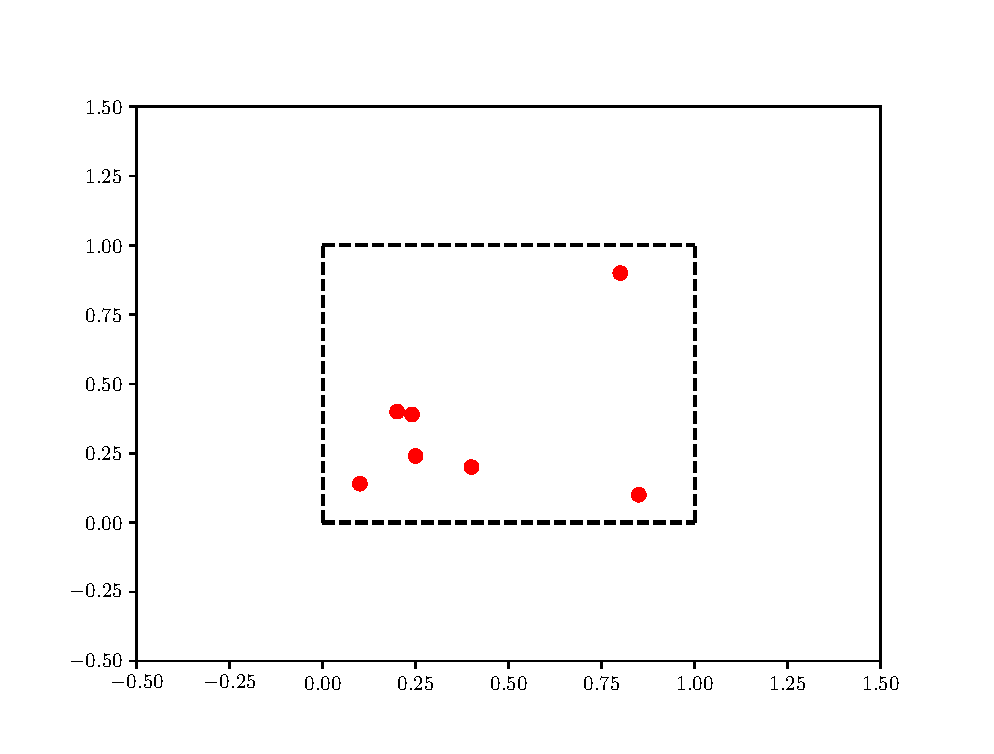
\includegraphics[width=\textwidth]{imbalanced-data.eps}
\end{column}
\end{columns}
\end{frame}

\begin{frame}\frametitle{What Could Go Wrong: Extrapolation}
\begin{columns}
\begin{column}{0.6\textwidth}
\begin{itemize}
\pause
\item ${\hat F}_{\cal T}$ is only defined in the ${\cal CH}({\cal P})$
\item Will have to project $q$ into ${\cal CH}({\cal P})$ and interpolate
projection
\item {\color{red} Low accuracy when residual is large}
\item When ${\cal CH}({\cal P})$ is a small subset of ${\cal X}$,
overall accuracy can be poor
\end{itemize}
\end{column}
\begin{column}{0.4\textwidth}
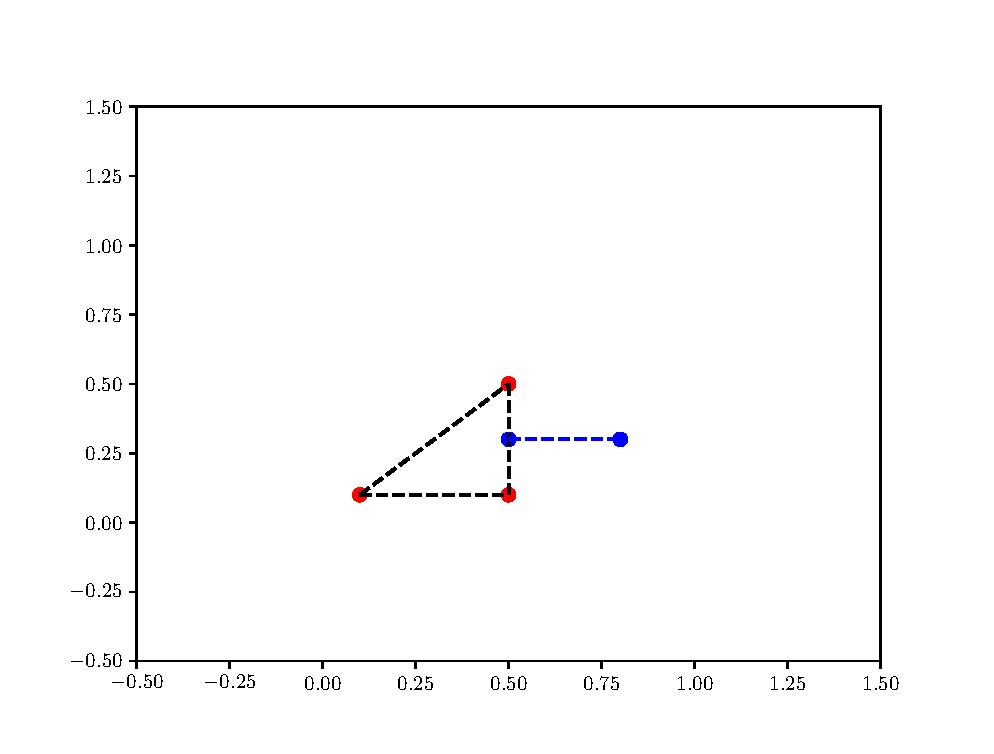
\includegraphics[width=\textwidth]{projection.eps}
\end{column}
\end{columns}
\end{frame}

\begin{frame}\frametitle{Same Issues for RBFs/GPs}
$$
{\hat F}_{RBF} =
\omega^\top \left[ \begin{array}{c}
e^{-\|x_1 - x\|^2/\sigma}\\
e^{-\|x_2 - x\|^2/\sigma}\\
\vdots\\
e^{-\|x_n - x\|^2/\sigma}
\end{array} \right]
$$
\pause
where
$ A \omega = y $
and 
$$
A = 
\left[
\begin{array}{cccc}
1 & e^{-\|x_1 - x_2\|^2/\sigma} & \ldots & e^{-\|x_1 - x_n\|^2/\sigma} \\
e^{-\|x_2 - x_1\|^2/\sigma} & 1 & \ldots & e^{-\|x_2 - x_n\|^2/\sigma} \\
\vdots & \vdots &  & \vdots \\
e^{-\|x_n - x_1\|^2/\sigma} & e^{-\|x_n - x_2\|^2/\sigma} & \ldots & 1 \\
\end{array}
\right]
\qquad
y = 
\left[
\begin{array}{c}
F(x_1) \\
F(x_2) \\
\vdots \\
F(x_n) \\
\end{array}
\right]
$$

\end{frame}

\begin{frame}\frametitle{RBF/GP Conditioning and Accuracy}
$$
A = 
\left[
\begin{array}{cccc}
1 & e^{-\|x_1 - x_2\|^2/\sigma} & \ldots & e^{-\|x_1 - x_n\|^2/\sigma} \\
e^{-\|x_2 - x_1\|^2/\sigma} & 1 & \ldots & e^{-\|x_2 - x_n\|^2/\sigma} \\
\vdots & \vdots &  & \vdots \\
e^{-\|x_n - x_1\|^2/\sigma} & e^{-\|x_n - x_2\|^2/\sigma} & \ldots & 1 \\
\end{array}
\right]
$$
\begin{itemize}
\pause \item As we seek higher accuracy, data points get closer together
\pause \item As $\|x_i - x_j\| \rightarrow 0$, $A \rightarrow$ singularity
\pause \item Decrease the shape parameter $\sigma$ to keep $A$ nonsingular
\pause \item Descreasing $\sigma$ restricts the support of ${\hat F}_{RBF}$
\begin{itemize}
\pause
\item Inability to extrapolate outside ${\cal CH}({\cal P})$
\item When data is imabalanced, accuracy will {\it decrease} in low density
regions
\end{itemize}
\pause \item ``Uncertainty principle'' -- for real-world datasets, cannot
have accuracy and solvability
\end{itemize}
\end{frame}

\begin{frame}\frametitle{More general with Fully Linear Models}

\pause
A fully linear model is ``accurate enough'' to use as a gradient oracle
in a $\delta$-ball around $x_0$

\pause
$$
\begin{array}{c}
|{\hat F}(x)-F(x)| \leq C_1 \delta^2\\
\| \nabla {\hat F}(x) - \nabla F(x)\| \leq C_2 \delta
\end{array}
$$

for all $\|x - x_0\| < \delta$.

\pause
\begin{itemize}
\item When ${\hat F}$ interpolates, conditions for fully linearity
reduce to geometric conditions
\begin{itemize}
\item $d+1$ model points in ball are affinely independent
\end{itemize}
\item Only accurate within ball
\begin{itemize}
\item no guarantees during extrapolation
\item no convergence in low-density regions
\end{itemize}
\end{itemize}
\end{frame}

\begin{frame}\frametitle{Summary of Bad Data}
\begin{itemize}
\item Small convex hull
\item Imbalanced
\item Poorly conditioned
\end{itemize}

\bigskip
\pause

Real-world datasets have zero-volume in high-dimensions, which leads to
all of the properties

\end{frame}

\section{A Proposed Solution}

\begin{frame}\frametitle{Design of Experiments}

\begin{itemize}
\pause \item Classical deterministic designs -- full-factorial, central composite, box-behnkin
\begin{itemize}
\item Typically don't scale well to many dimensions
\end{itemize}
\pause \item Optimal design of experiments -- A-optimal, E-optimal, D-optimal designs
\begin{itemize}
\item Maximize info gain, which is roughly equivalent to max.~model conditioning
\item Expensive to calculate
\item Typically require a model {\sl a priori}
\end{itemize}
\pause \item Geometric criteria -- maximin and minimax
\begin{itemize}
\item Heuristically good for maximizing convex hulls
\item Expensive to calculate in high dimensions
\end{itemize}
\pause \item Low discrepancy sequences -- Sobol, Halton, etc.
\begin{itemize}
\item Produce balanced datasets
\item Performance falls off when sample size is not chosen carefully
\end{itemize}
\pause \item Latin hypercubes
\begin{itemize}
\item Stratifies sample -- good for linear models
\item No theory for nonlinear models
\item Heuristically good in practice and cheap to calculate
\end{itemize}
\end{itemize}
\end{frame}

\begin{frame}\frametitle{Stochastic Fourier SFD}
\begin{columns}
\begin{column}{0.3\textwidth}
\begin{center}
\begin{tabular}{l}
 - Desired sample size\\
 - Performance criertia
\end{tabular}\\

\bigskip
\bigskip
\bigskip
\bigskip
\bigskip

{\tt COBYLA}

\end{center}
\end{column}
\begin{column}{0.2\textwidth}

$\xrightarrow{\hspace*{1.5cm}}$\\

\medskip
\bigskip
\bigskip
\bigskip
\bigskip
\bigskip

$\xleftarrow{\hspace*{1.5cm}}$\\

\end{column}
\begin{column}{0.3\textwidth}
\begin{center}
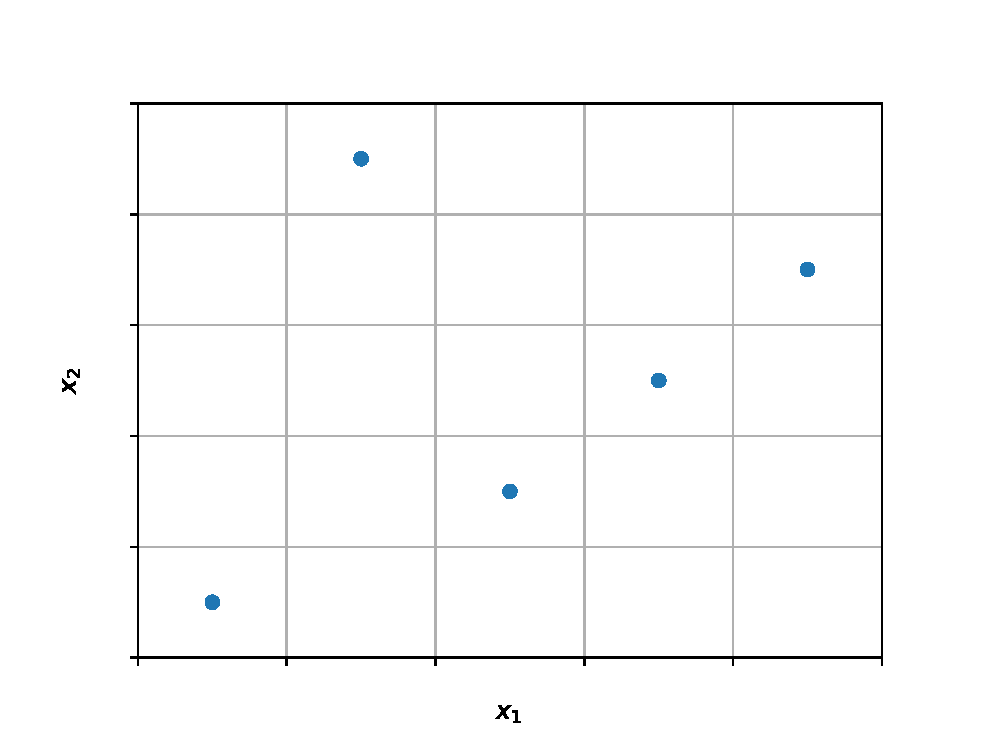
\includegraphics[width=0.6\textwidth]{lh_doe.eps}\\

$\downarrow$\\

$$
\alpha_1 e^{2\pi i x} + \alpha_2 e^{2 \pi i (2x)} + \ldots
$$
\end{center}
\end{column}
\end{columns}
\end{frame}

\begin{frame}\frametitle{Preliminary Results}
\begin{columns}
\begin{column}{0.3\textwidth}
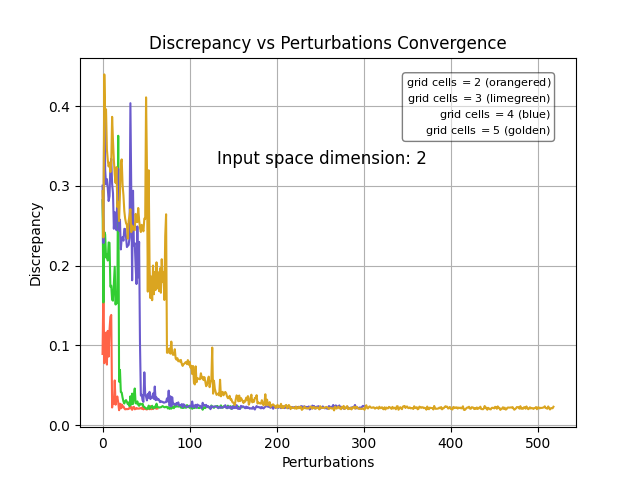
\includegraphics[width=\textwidth]{2.png}\\
\end{column}
\begin{column}{0.3\textwidth}
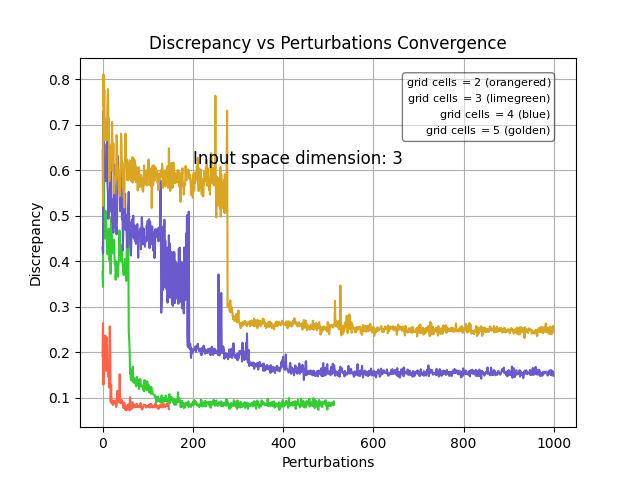
\includegraphics[width=\textwidth]{3.png}\\
\end{column}
\begin{column}{0.3\textwidth}
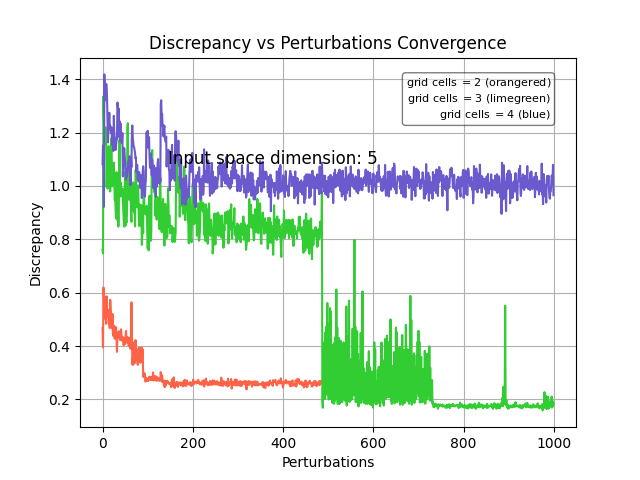
\includegraphics[width=\textwidth]{5.png}\\
\end{column}
\end{columns}
\end{frame}

\begin{frame}\frametitle{Resources}
\begin{center}
{\large
E-mail: {\tt tchang@anl.gov}}\\
\bigskip
\bigskip
Code: {\tt github.com/thchang/sf-sfd}\\

\bigskip
\bigskip

{\small This material is based upon work supported by the U.S. Department of Energy, Office of Science, Office of Advanced Scientific Computing Research, SciDAC program under contract number DE-AC02-06CH11357.}
\end{center}
\end{frame}

\end{document}
